\documentclass[handout]{beamer}
\usepackage{array}
\usepackage{german}
\usepackage{graphicx}
\usepackage[utf8]{inputenc}
\usepackage[T1]{fontenc}
\mode<beamer>{%
\usetheme{Copenhagen}
}
\usepackage[orientation=landscape,size=a3,debug,scale=2.5]{beamerposter}
\title[]{}
\begin{document}
\begin{frame}
\frametitle{%\hspace{0pt plus 1 filll}
MathSem 2022: Spezielle Funktionen}
\begin{columns}[t,onlytextwidth]
\begin{column}{0.32\textwidth}
%{%\bf
%\large Das Buch zum Seminar}
%\bigskip
%\vskip 1cm
\begin{center}
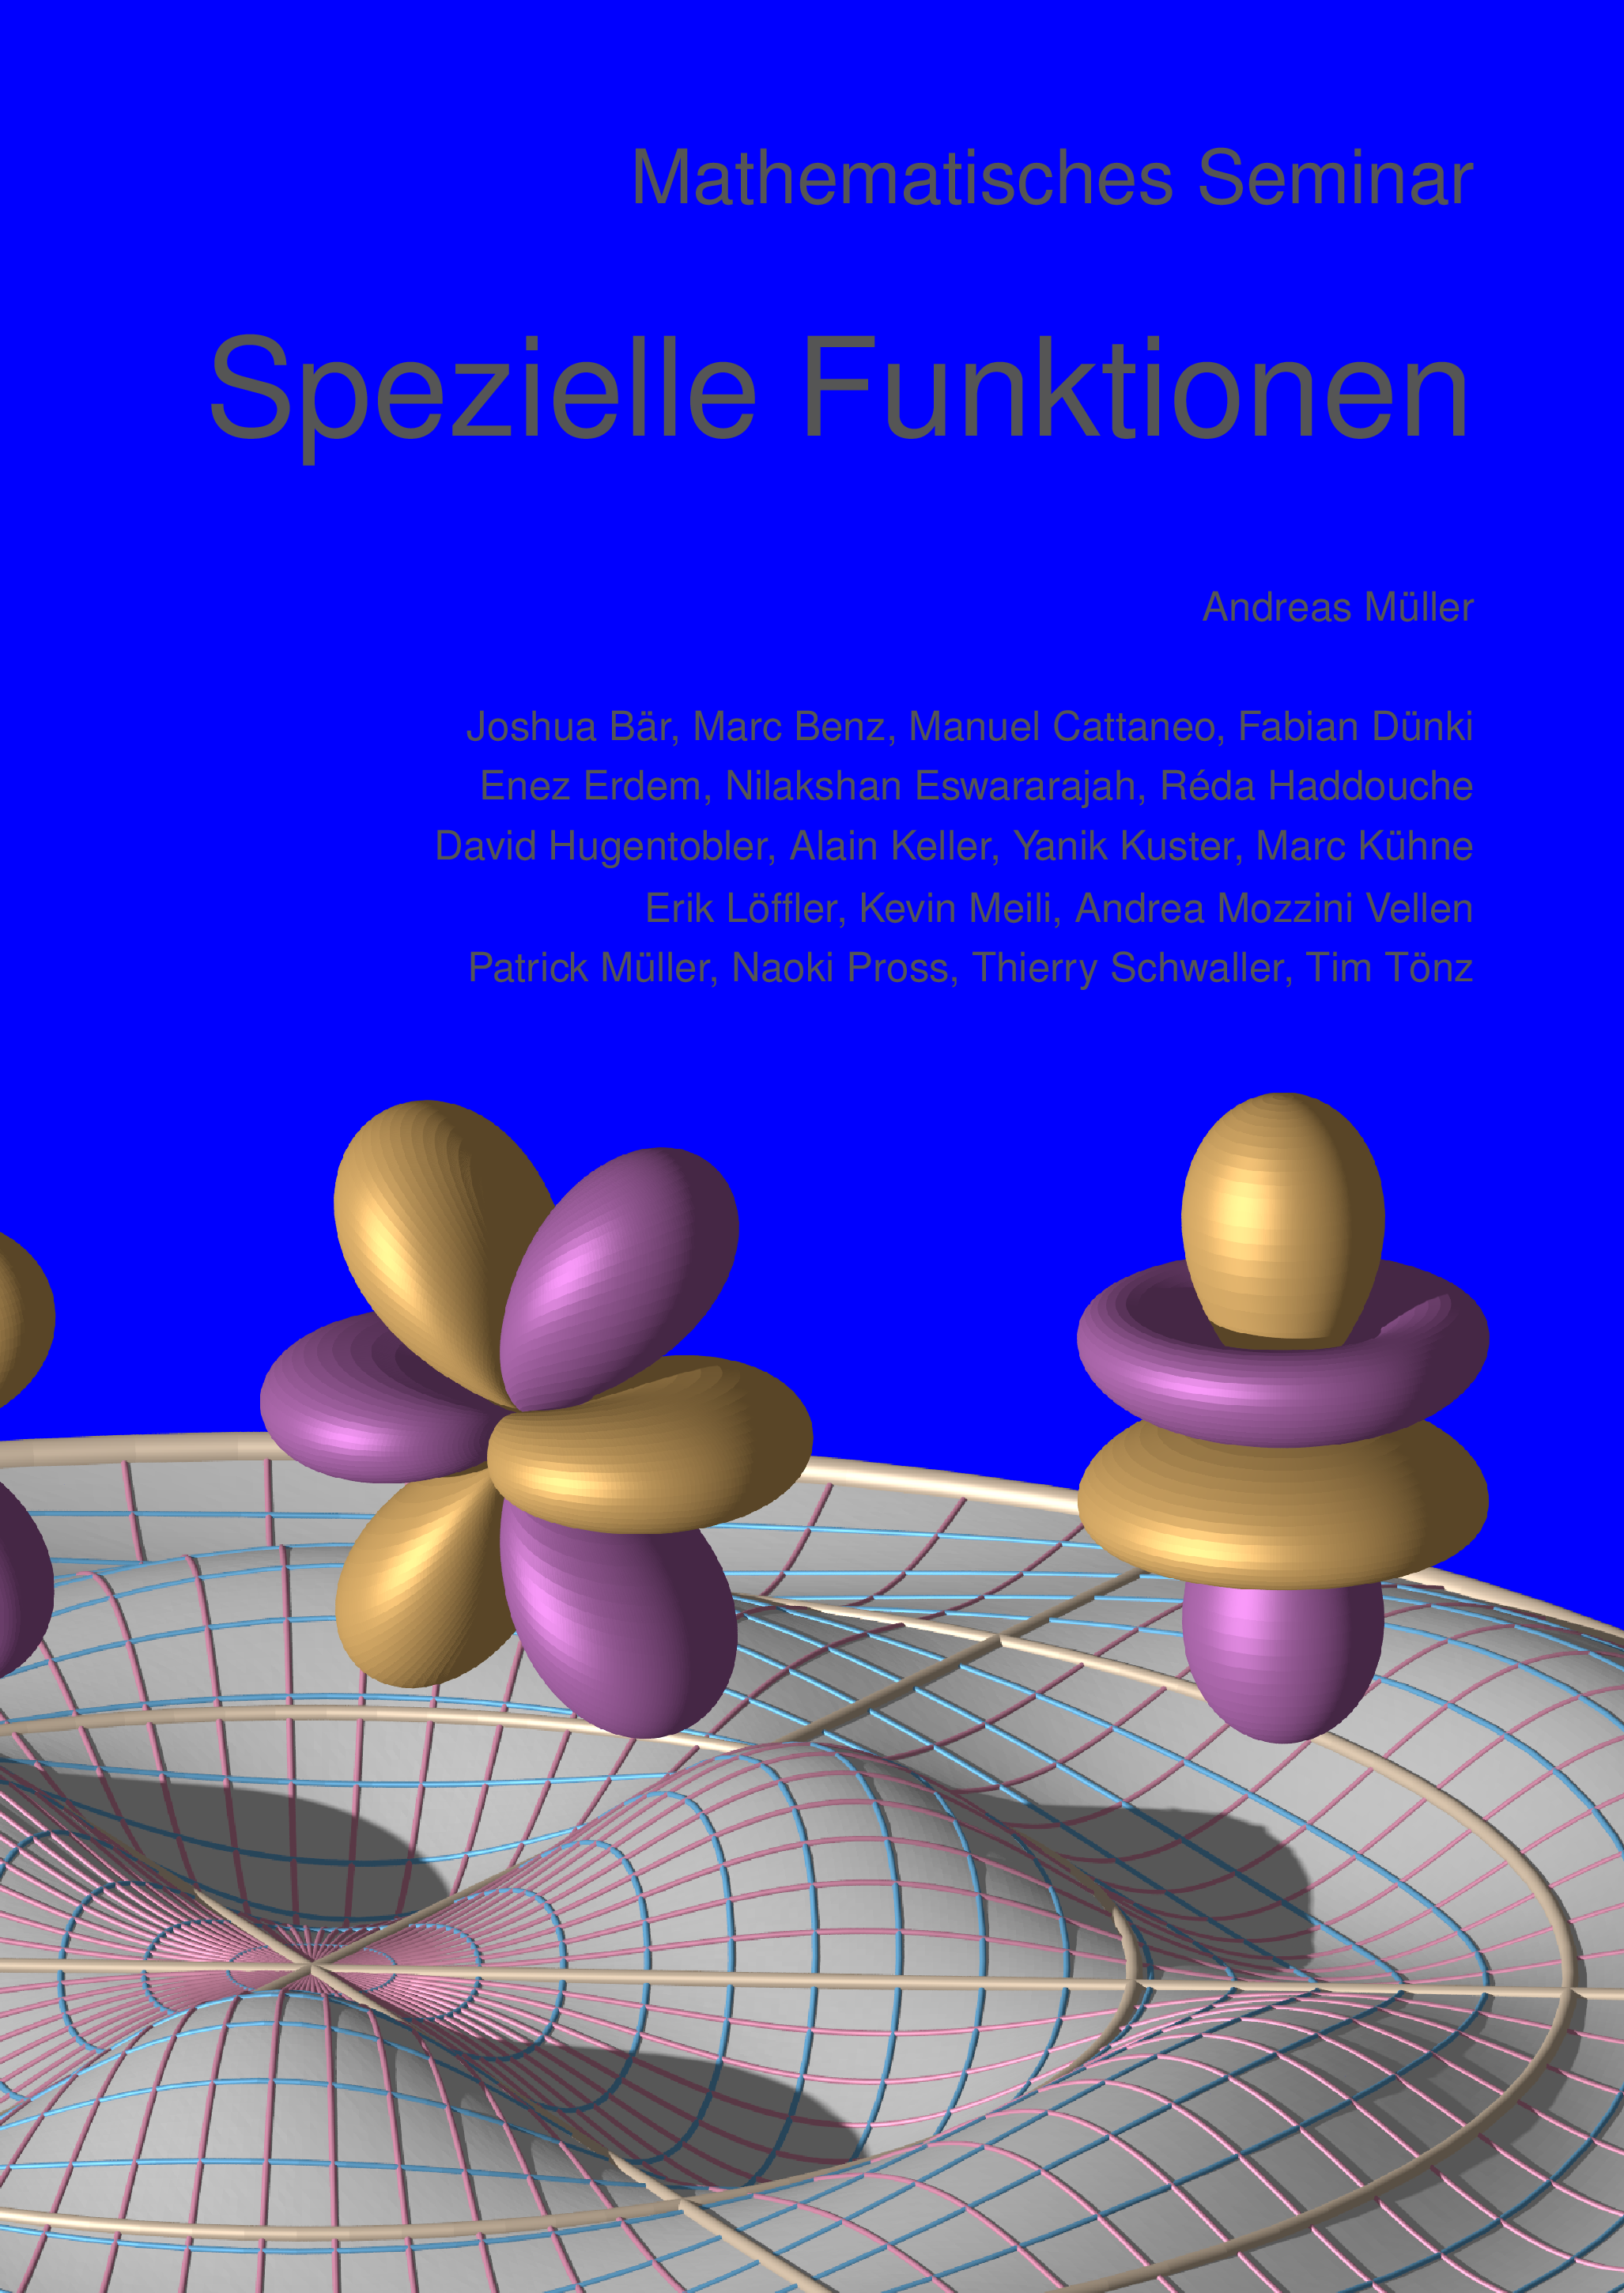
\includegraphics[width=\hsize]{../cover/buchcover.png}
\end{center}
\vskip 0.2cm
\bigskip
\bigskip
Erscheint~im~Herbst~2022.\\
Anfragen~an~Prof.~Dr.~Andreas Müller,\\
{\texttt{andreas.mueller@ost.ch}}
\bigskip
\bigskip
\bigskip
%\vskip 1.2cm
\end{column}
\begin{column}{0.65\textwidth}
\begin{description}
\item[Teil 1:] Grundlagen
\begin{enumerate}
\item Potenzen und Wurzeln
\item Exponentialfunktion und Exponentialgleichungen
\item Spezielle Funktionen aus der Geometrie
\item Spezielle Funktionen und Rekursion
\item Differentialgleichungen
\item Integrale
\item Orthogonalität
\item Funktionentheorie
\item Partielle Differentialgleichungen
\item Integraltransformationen
\item Elliptische Funktionen
\end{enumerate}
\item[Teil 2:] Anwendungen und weiterführende Themen
\begin{enumerate}
\setcounter{enumi}{11}
\item David Hugentobler und Yanik Kuster: {\em Verfolgungskurven}
\item Joshua Bär: {\em Frequenzmodulation und Bessel-Funktionen}
\item Alain Keller und Thierry Schwaller: {\em Parabolische Zylinderfunktionen}
%\item Andreas Müller: {\em Fresnel-Integrale}
\setcounter{enumi}{15}
\item Andrea Mozzini Vellen und Tim Tönz: {\em Schwingungen einer kreisförmigen Membran}
\item Réda Haddouche und Erik Löffler: {\em Sturm-Liouville-Probleme}
\item Patrik Müller: {\em Laguerre-Polynome}
\item Raphael Unterer: {\em Riemannsche Zeta-Funktion}
\item Fabian Dünki: {\em Algorithmus zur Berechnung von $\mathstrut_0F_1$}
\item Enez Erdem und Marc Kühne: {\em Sphärische Navigation}
\item Marc Benz: {\em Transferfunktion Tangens Hyperbolicus}
\item Samuel Niederer: {\em Riccati-Differentialgleichung}
\item Manuele Cattaneo und Naoki Pross: {\em Spherical Harmonics}
\item Nicolas Tobler: {\em Elliptische Filter}
%\item Andreas Müller: {\em $\int P(t)e^{-t^2}\,dt$ in geschlossener Form?}
\end{enumerate}
\end{description}
\end{column}
\begin{column}{0.01\textwidth}
\llap{\raisebox{-3cm}{\includegraphics{qrcode.pdf}}}
\end{column}
\end{columns}
\end{frame}
\end{document}
